
%-----------------------------------------------------------------------
\subsection{The Group Algebra $\CG$}
%-----------------------------------------------------------------------
\label{sec:groupalgebra}
The \emph{group algebra} $\CG$ is the space of all formal sums
\begin{equation}
f = \sum_{x\in G} f(x) x, \quad f(x) \in \C,
\end{equation}
with the following operations for $f, g \in \CG$:
\begin{equation}
f+g = \sum_{x\in G} (f(x) + g(x))x,
\end{equation}
\begin{equation}
\alpha f = \sum_{x\in G} (\alpha f(x)) x, 
           \quad \alpha \in \C,
\end{equation}
\begin{equation}
fg = \sum_{x\in G}\left(\sum_{y\in G} f(y)g(y^{-1}x)\right)x. 
\end{equation}

The mapping $\lt{L}(g)$ of $\CG$ defined by 
$\lt{L}(g)f = gf$
is a linear operator on the space $\CG$ called 
\emph{left multiplication by} $g$.  
Since $y\in G$ can be identified with the formal
sum $e_y \in \CG$ consisting of a single nonzero term,
\begin{equation}\label{eq:leftmult}
yf = \lt{L}(e_y)f = \sum_{x\in G}f(y^{-1}x) x.
\end{equation}
In relation to translation of $\LG$, (\ref{eq:leftmult}) is the
$\CG$ analog. Fig.~\ref{fig:cyclicshift} illustrates.

The mapping $\Theta: \LG \to \CG$ defined by
\begin{equation}\label{eq:iso}
\Theta(f) = \sum_{x\in G} f(x) x, \quad f\in \LG,
\end{equation}
is an algebra isomorphism of the convolution algebra $\LG$
onto the group algebra $\CG$.  
Thus we can identify
$\Theta(f)$ with $f$, using  context to decide whether
$f$ refers to the function in $\LG$ or the formal sum in
$\CG$.  

An important aspect of the foregoing isomorphism is the
correspondence between the translations of the spaces.
Translation of $\LG$ by $y\in G$ %$\T(y)$ 
corresponds to left multiplication of $\CG$ by $y\in G$.
%$\lt{L}(y)$ 
Convolution of $\LG$ by $f\in \LG$ corresponds to
left multiplication of $\CG$ by $f\in \CG$. 
%We state 
%these relations symbolically as follows:
%\begin{center}
%\begin{tabular}{ccc}
%  $\LG$ & $\simeq$ & $\CG$ \\
%  $\lt{T}(y)$ & $\leftrightarrow$ & $\lt{L}(y)$\\
%  $\lt{C}(f)$ & $\leftrightarrow$ & $\lt{L}(f)$
%\end{tabular}
%\end{center}

\begin{figure}
\centerline{\framebox{
	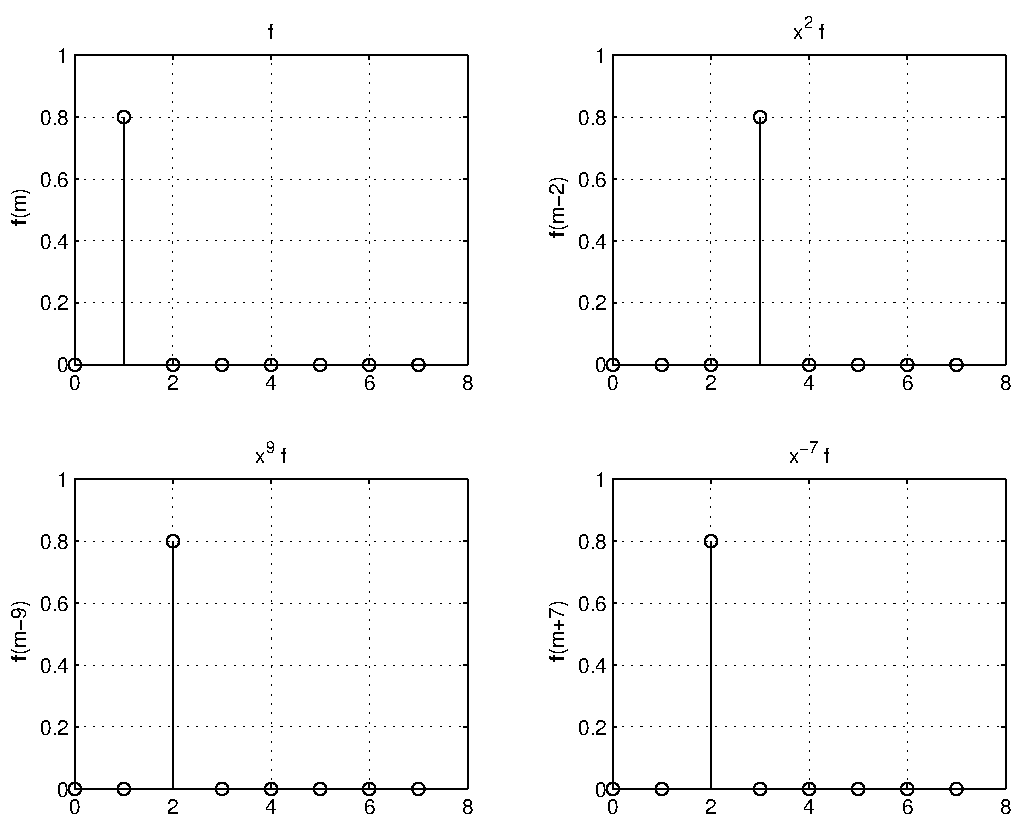
\includegraphics[width=\columnwidth]{t_cyclicshift}}}
  \caption{An impulse $f\in \CA$ and a few abelian group translates, $x^2f, x^9f,
      x^{-7}f$.}
  \label{fig:cyclicshift}
\end{figure}

%\begin{figure}
%%  \centerline{\epsfig{figure=figures/t_cyclicshift,width=70mm, height=50mm}}
%  \centering
%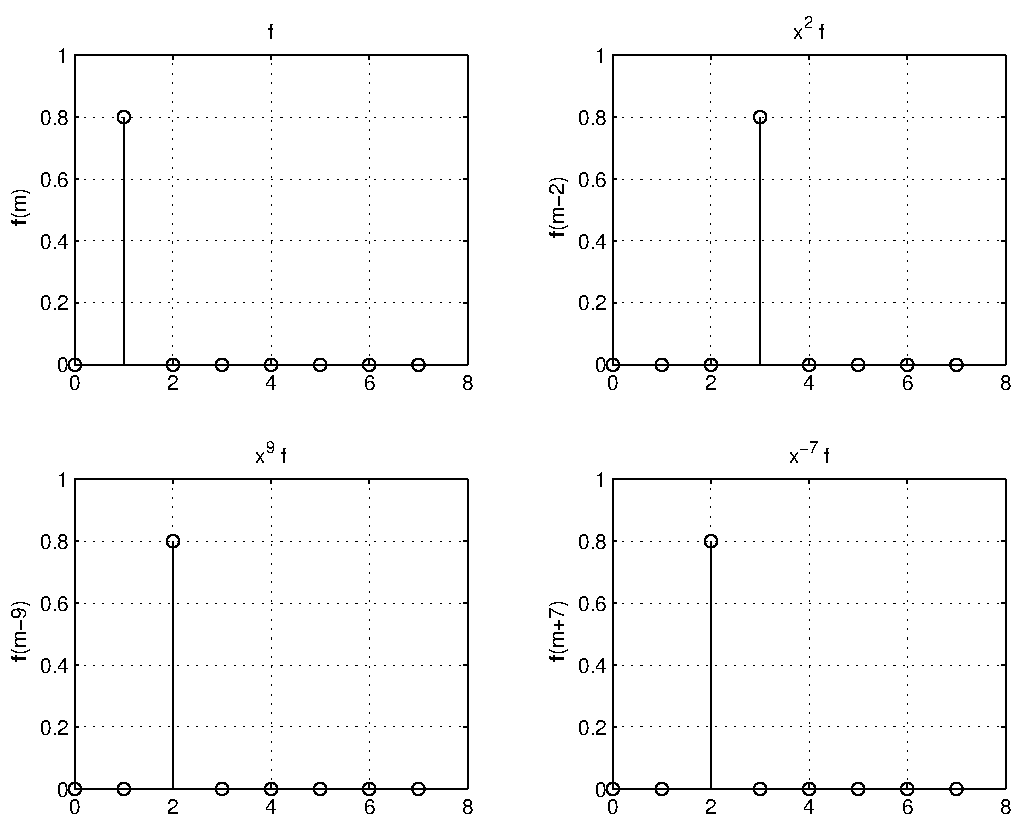
\includegraphics[width=80mm, height=70mm]{t_cyclicshift}
%  \caption{An impulse $f\in \CA$ and a few abelian group translates, $x^2f, x^9f,
%      x^{-7}f$.}
%  \label{fig:cyclicshift}
%\end{figure}

%------------------------------------------------------------------------
\subsection{Ideals: Translation-Invariant Subspaces}
%------------------------------------------------------------------------
A subspace $\vs{V}$ of the space $\CG$ is called a
\emph{left ideal} if 
\begin{equation}
u\vs{V} = \{uf : f \in \vs{V}\} \subset \vs{V}, \quad u \in G. 
\end{equation}
A left ideal of $\CG$ corresponds to a subspace of $\LG$
invariant under all left translations.  

If $\vs{V}$ is a left ideal, then, by linearity, 
$g\vs{V} \subset \vs{V}$ for all $g \in \CG$.
The set $\CG g$, defined by 
$\{fg : f \in \CG\}$, is a left ideal of $\CG$,
called \emph{the left ideal generated by} $g$ in $\CG$. 
%$\CG g = \CG$ if and only if $g$ is an invertible element in $\CG$. 
A left ideal $\vs{V}$ of $\CG$ is called \emph{irreducible}
if the only left ideals of $\CG$ contained in $\vs{V}$ are
$\{0\}$ and $\vs{V}$. The sum of two distinct, irreducible
left ideals is always a direct sum. 
% (\cite{An:2003}, p.~129).

For \emph{abelian} group $A$, the group algebra $\C A$ of
signals is decomposed into a direct sum of irreducible ideals.  
Since multiplication of $\C A$ by elements of $A$
corresponds to translation, ideals represent
translation-invariant subspaces.  Furthermore, in the 
abelian case, such translation-invariant subspaces are
one-dimensional.   

Similarly, for \emph{nonabelian} group $G$, the group algebra
$\CG$ is decomposed into a direct sum of left ideals. Here,
again, the ideals are translation-invariant 
subspaces.  However, some of these subspaces must now be
multi-dimensional, and herein lies the potential advantage
of using nonabelian groups for indexing the data. The left
translations are more general and represent a broader class of 
transformations. Therefore, projections of data into the
resulting left ideals can reveal more complicated partitions
and structures in the data as compared with the Fourier
components in the abelian group case. 
